\documentclass[11pt,oneside]{article}

\usepackage[a4paper,margin=25mm,headheight=22pt]{geometry}
\usepackage[T1]{fontenc}
\usepackage[utf8]{inputenc}
\IfFileExists{libertinus.sty}{\usepackage{libertinus}}{\usepackage{lmodern}}
\usepackage{microtype}
\usepackage{amsmath,amssymb,amsthm,mathtools,mathrsfs,bm}
\usepackage{booktabs,longtable,tabularx,array,multirow}
\usepackage{graphicx}
\usepackage{float}
\usepackage{xcolor}
\usepackage{enumitem}
\usepackage{fancyhdr}
\usepackage{titlesec}
\usepackage{xurl}
\usepackage{listings}
\usepackage{fancyvrb}
\usepackage{hyperref}
\usepackage[nameinlink,noabbrev]{cleveref}

\definecolor{DeepBlue}{RGB}{28,65,104}
\definecolor{Teal}{RGB}{25,112,111}
\definecolor{Burgundy}{RGB}{132,48,61}
\definecolor{Gold}{RGB}{164,112,28}
\definecolor{SoftGray}{RGB}{246,247,249}
\definecolor{RuleGray}{RGB}{194,202,210}
\definecolor{DarkGreen}{RGB}{25,101,64}

\hypersetup{
  colorlinks=true,
  linkcolor=DeepBlue,
  citecolor=DarkGreen,
  urlcolor=Teal,
  pdftitle={Confluent Digital Extrapolation and Lambert-Phase Tomography in the Fabius--Rvachev System},
  pdfauthor={Research synthesis for Vladimir Reshetnikov},
  pdfsubject={New frontier results for the Fabius function, inverse Fabius function, Rvachev up-function, Thue--Morse sequence, q-binomial extrapolation, Lambert W, Bell and Bernoulli polynomials},
  pdfkeywords={Fabius function, inverse Fabius function, Rvachev up-function, Thue-Morse, Richardson extrapolation, q-binomial, Lambert W, Bell polynomial, Bernoulli polynomial, Gamma zeta}
}
\urlstyle{same}

\pagestyle{fancy}
\fancyhf{}
\fancyhead[L]{\small\color{DeepBlue}Confluent digital extrapolation}
\fancyhead[R]{\small\color{Teal}Fabius--Rvachev frontier report}
\fancyfoot[C]{\small\thepage}
\renewcommand{\headrulewidth}{0.35pt}
\renewcommand{\headrule}{\hbox to\headwidth{\color{RuleGray}\leaders\hrule height \headrulewidth\hfill}}

\titleformat{\section}{\Large\bfseries\color{DeepBlue}}{\thesection}{0.70em}{}
\titleformat{\subsection}{\large\bfseries\color{DeepBlue}}{\thesubsection}{0.65em}{}
\titleformat{\subsubsection}{\normalsize\bfseries\color{Teal}}{\thesubsubsection}{0.60em}{}
\setcounter{secnumdepth}{3}
\setcounter{tocdepth}{2}
\numberwithin{equation}{section}
\allowdisplaybreaks[3]
\setlength{\emergencystretch}{3em}
\setlist[itemize]{leftmargin=1.8em,itemsep=0.24em,topsep=0.4em}
\setlist[enumerate]{leftmargin=2.15em,itemsep=0.24em,topsep=0.4em}

\newtheorem{theorem}{Theorem}[section]
\newtheorem{proposition}[theorem]{Proposition}
\newtheorem{lemma}[theorem]{Lemma}
\newtheorem{corollary}[theorem]{Corollary}
\newtheorem{conjecture}[theorem]{Conjecture}
\newtheorem{problem}[theorem]{Open problem}
\theoremstyle{definition}
\newtheorem{definition}[theorem]{Definition}
\newtheorem{algorithm}[theorem]{Algorithm}
\newtheorem{example}[theorem]{Example}
\theoremstyle{remark}
\newtheorem{remark}[theorem]{Remark}
\newtheorem{warning}[theorem]{Warning}

\newcommand{\R}{\mathbb R}
\newcommand{\C}{\mathbb C}
\newcommand{\N}{\mathbb N}
\newcommand{\Z}{\mathbb Z}
\newcommand{\Q}{\mathbb Q}
\newcommand{\e}{\mathrm e}
\newcommand{\ii}{\mathrm i}
\newcommand{\dd}{\,\mathrm d}
\newcommand{\bigO}{\mathcal O}
\newcommand{\smallo}{o}
\newcommand{\Up}{\operatorname{up}}
\newcommand{\sinc}{\operatorname{sinc}}
\newcommand{\supp}{\operatorname{supp}}
\newcommand{\sgn}{\operatorname{sgn}}
\newcommand{\wt}{s_2}
\newcommand{\vtwo}{\nu_2}
\newcommand{\DFT}{\operatorname{DFT}}
\newcommand{\Res}{\operatorname*{Res}}
\newcommand{\qbinom}[3]{\genfrac{[}{]}{0pt}{}{#1}{#2}_{#3}}
\newcommand{\ThetaTM}{\Theta_{\!\mathrm{TM}}}
\newcommand{\Bell}{\mathcal B}
\newcommand{\Wiener}{\mathcal A}
\newcommand{\repo}{\textsc{ProveIt}}
\newcommand{\statusproved}{\textcolor{DarkGreen}{\textbf{proved here}}}
\newcommand{\statusderived}{\textcolor{DeepBlue}{\textbf{derived from audited corpus inputs}}}
\newcommand{\statusopen}{\textcolor{Burgundy}{\textbf{conjectural/open}}}

\newenvironment{resultbox}[1]{%
  \par\medskip\noindent\begin{center}\begin{minipage}{0.94\textwidth}%
  \color{Teal}\hrule height 0.8pt\vspace{0.6em}%
  \color{black}\textbf{\color{Teal}#1.}\ }{%
  \par\vspace{0.6em}\color{Teal}\hrule height 0.55pt
  \end{minipage}\end{center}\medskip}

\newenvironment{statusbox}[1]{%
  \par\medskip\noindent\begin{center}\begin{minipage}{0.94\textwidth}%
  \color{DeepBlue}\hrule height 0.8pt\vspace{0.6em}%
  \color{black}\textbf{\color{DeepBlue}#1.}\ }{%
  \par\vspace{0.6em}\color{DeepBlue}\hrule height 0.55pt
  \end{minipage}\end{center}\medskip}

\newenvironment{conjecturebox}[1]{%
  \par\medskip\noindent\begin{center}\begin{minipage}{0.94\textwidth}%
  \color{Gold}\hrule height 0.8pt\vspace{0.6em}%
  \color{black}\textbf{\color{Gold}#1.}\ }{%
  \par\vspace{0.6em}\color{Gold}\hrule height 0.55pt
  \end{minipage}\end{center}\medskip}

\lstdefinestyle{code}{
  language=Python,
  basicstyle=\ttfamily\footnotesize,
  backgroundcolor=\color{SoftGray},
  frame=single,
  rulecolor=\color{RuleGray},
  breaklines=true,
  columns=fullflexible,
  keepspaces=true,
  showstringspaces=false,
  keywordstyle=\color{DeepBlue}\bfseries,
  commentstyle=\color{Teal},
  stringstyle=\color{Burgundy},
  xleftmargin=0.6em,xrightmargin=0.6em,
  aboveskip=0.8em,belowskip=0.8em
}

\title{\bfseries Confluent Digital Extrapolation and\\[0.18em]
Lambert-Phase Tomography\\[0.28em]
\large in the Fabius--Rvachev System\\[0.55em]
\normalsize Repeated spectral roots, bounded Thue--Morse filters, maximal Gamma--zeta strips,\\
and two-axis recovery of periodic endpoint coefficients}
\author{Research synthesis prepared for Vladimir Reshetnikov\\
\small after a recursive audit of the complete \texttt{*.tex} corpus under\\
\path{Analysis/FabiusFunction/docs}}
\date{Pinned repository snapshot: 27 August 2026\\
\small commit \texttt{f49aad5c9c6d627a64822ea9f8e46f5270b95cef}}

\begin{document}
\maketitle

\begin{abstract}
The audited \repo{} corpus already contains the classical and formalized theory of the
Fabius function and Rvachev's up-function, exact dyadic values, inverse endpoint
asymptotics, Gaussian $q$-binomial interpolation, Bernoulli cumulants, Bell-polynomial
saddle coefficients, sharp real-axis decay of the infinite sinc product, spectral zero
multiplicities, the Pascal--Rvachev hierarchy, logarithmic $q$-Richardson acceleration,
and additive Lambert-phase locking.  The recursive tree at the pinned commit contains
78 LaTeX paths, including historical revisions, imported papers, and six generated table
fragments.  These materials were treated as one revision-aware corpus; established
results are not relabeled as discoveries here.

This report develops a different theorem package.  First, for a sequence containing
polynomially decorated geometric modes $n^\ell q^n$, a normalized shift polynomial with
a root of multiplicity $m$ at $q$ annihilates all decorations with $\ell<m$.  The unique
minimal-degree filter, its exact condition number, its Banach-valued remainder bound, and
its mixed-mode extension are obtained in closed form.  The familiar Gaussian
$q$-Richardson row is precisely the simple-root specialization.

Second, a nonminimal factorization gives a surprising stability improvement.  Twisting a
length-$2^m$ Thue--Morse block by $q^{-n}$ produces a filter of order $m$ whose
$\ell^1$ condition number is
\[
 \kappa_m^{\rm TM}(q)
 =\frac{1-q^{2^m}}{(1-q)\prod_{j=0}^{m-1}(1-q^{2^j})}
 \longrightarrow \frac{1}{(1-q)\ThetaTM(q)}.
\]
Thus the cancellation order tends to infinity while the condition number stays bounded.
For $q=1/2$ the limit is approximately $5.7112854057$, whereas the minimal repeated-root
filter has condition number $3^m$.  The price is a stencil span $2^m-1$.  The powers of
two are characterized as the unique minimal-span collision-free factorization.

Third, in the exact lower-Lambert coordinate $x=\lambda2^{-\lambda}$, every rational phase
$\theta=a/d$ has multiplicative locks
$\lambda_s=\rho^s(n+\theta)$ whenever $\rho\equiv1\pmod d$.  Inverse powers become
geometric modes and logarithmically decorated inverse powers become confluent geometric
modes.  This converts endpoint extraction into a stable $q$-Richardson problem with
bounded weights, contrasting sharply with the polynomially growing condition number of
the corpus's additive locks $\lambda+j$.

Fourth, the corpus's exact Gamma--zeta formula for the leading periodic endpoint term is
shown to imply the exact maximal holomorphy strip
\[
 |\Im z|<\frac{\pi}{2\log2}.
\]
Weighted Wiener-algebra bounds then make Bell-polynomial and derivative constructions
quantitatively stable.  Combining radial multiplicative extrapolation with a discrete
Fourier transform over rational phases yields a two-axis tomography algorithm: radial
error is algebraic in the starting Lambert coordinate, while angular aliasing is
exponentially small at the sharp rate $\pi^2/\log2$.

All theorem statements are proved in the report.  Claims about natural boundaries,
optimal span--conditioning tradeoffs, irrational near-locks, and resurgent late-order
behavior are explicitly labeled conjectural.  The accompanying Python program performs
exact rational cancellation checks and high-precision Gamma--zeta experiments and
regenerates every table and figure.
\end{abstract}

\begin{statusbox}{Proof and novelty convention}
``Proved here'' means proved in this manuscript, not yet formalized in Lean.  ``New'' means
not found as an exact theorem or construction in the pinned 78-path corpus after path,
phrase, formula, and structural searches.  It is deliberately not a claim of worldwide
priority.  The endpoint expansion and its Gamma--zeta Fourier formula are audited inputs;
the confluent filters, digital stability theorem, rational multiplicative phase geometry,
maximal-strip consequence, and two-axis tomography are the new deductions.
\end{statusbox}

\tableofcontents
\clearpage

\section{Corpus boundary and nonduplication audit}
\label{sec:audit}

\subsection{Pinned recursive inventory}

The default branch changed during the audit, so all comparisons use the immutable commit
printed on the title page.  Its documentation subtree has recursive Git tree SHA
\path{6063d0d90cd9a4d25ca74cd4f8b80448313fce64}.  The tree contains 78 LaTeX
paths.  GitHub's code-search index returned fewer paths at several points because large,
recent, and generated files had not all been indexed; the recursive tree, not code search,
was therefore the inventory authority.

The corpus consists of current expositions, frozen revisions, a consolidated frontier
volume, numerous current frontier reports, twelve Fourier-decay dossiers, source-paper
transcriptions, and six small TeX fragments generated for tables or checks.  Historical
revisions were read as mathematical lineages: a corrected successor supersedes an older
normalization, but a distinctive result surviving only in an archive file still counts as
prior art.  The complete path list is reproduced verbatim in \cref{app:inventory} and is
also supplied as \path{corpus_manifest.txt} \cite{proveit}.

\subsection{Strong negative controls}

The following attractive results are already present in the corpus and are therefore
excluded from the novelty claims of this report:
\begin{itemize}
\item the probability model for $F$ and $\Up$, the dyadic sinc product, and the integer-zero
      multiplicity $1+\vtwo(n)$;
\item exact dyadic evaluation, $q=1/2$ Pochhammer and Gaussian-binomial formulas, Lagrange
      interpolation, and the standard simple-root $q$-Richardson row;
\item Prouhet cancellation and the finite Thue--Morse block product;
\item Bernoulli cumulants, Bell-polynomial moment and saddle calculations, Appell
      deconvolution, and Barnes-type finite-prefix formulas;
\item the corrected exact-Lambert endpoint coordinate, its nonconstant periodic term,
      all-orders inverse-power expansion, and additive phase-locked nodes $\lambda+j$;
\item logarithmic Richardson acceleration of truncated sinc products and its exact
      Gaussian-$q$-binomial error series;
\item the full Fourier zero divisor, spectral determinant and zeta, arithmetic rays,
      half-integer identities, local zero jets, and Pascal--Rvachev hierarchy;
\item positive self-sampling quadrature, alias superconvergence, and finite dyadic
      $q$-Richardson recovery;
\item sharp pointwise, metric, arithmetic, and envelope results for the real-axis infinite
      sinc product.
\end{itemize}

In particular, this report does \emph{not} claim ordinary geometric $q$-Richardson
extrapolation, Thue--Morse Prouhet cancellation, or Lambert phase locking separately.  Its
new contribution is the confluent and digitally factorized synthesis, together with the
new multiplicative phase geometry and the spectral regularity consequences.

\subsection{Result ledger}

\small
\begin{longtable}{@{}>{\raggedright\arraybackslash}p{0.07\textwidth}>{\raggedright\arraybackslash}p{0.66\textwidth}>{\raggedright\arraybackslash}p{0.19\textwidth}@{}}
\toprule
ID & Statement & Status\\
\midrule
\endhead
A & Shift-polynomial calculus for $n^\ell q^n$, unique minimal confluent
annihilator, exact $\ell^1$ condition number, and Banach-valued remainder bound.
& \statusproved\\
B & General Prouhet--Richardson factorization and the twisted Thue--Morse filter
with bounded infinite-order conditioning. & \statusproved\\
C & Minimal-span characterization of the binary exponents among collision-free
subset-product factorizations. & \statusproved\\
D & Rational multiplicative Lambert phase locks and confluent cancellation of
$\lambda^{-r}(\log\lambda)^\ell$ terms. & \statusproved\\
E & Exact comparison of additive and multiplicative phase-lock conditioning.
& \statusproved\\
F & Exact exponential type and maximal horizontal holomorphy strip of the leading
Gamma--zeta periodic endpoint term. & \statusderived\\
G & Radial $q$-interpolation of the periodic coefficient jet and angular DFT
alias formula with a combined error theorem. & \statusproved\\
H & Weighted Wiener-algebra and Bell-polynomial bounds for certified Fourier
truncation of all differential-polynomial endpoint coefficients. & \statusproved\\
I & Boundary naturality, optimal span--conditioning laws, irrational near-locks,
and late-order resurgence. & \statusopen\\
\bottomrule
\end{longtable}

\section{Established framework and normalization}
\label{sec:framework}

Only the audited inputs needed later are recalled.  Let $F$ be the bounded Fabius
distribution function on $[0,1]$, and let
\[
 \Up(x)=F(1-|x|),\qquad |x|\le1,
\]
with zero extension outside $[-1,1]$.  Under the Fourier convention used in the
primary exposition,
\begin{equation}
 \Phi(z)=\widehat\Up(z)
 =\prod_{h=0}^{\infty}\sinc\!\left(\frac{\pi z}{2^h}\right),
 \qquad \sinc w=\frac{\sin w}{w}.
 \label{eq:up-product}
\end{equation}
The product is entire; its nonzero integer zero at $n$ has multiplicity
$1+\vtwo(n)$.  Its logarithmic coefficients, cumulants, dyadic values, and large
real-axis behavior are developed extensively in the source corpus and the relevant
primary literature \cite{arias1982,arias2017,aistleitner2015,proveit}.

For the endpoint, put
\begin{equation}
 L=\log2,
 \qquad
 \lambda(x)=-\frac1L W_{-1}(-Lx).
 \label{eq:lambda-def}
\end{equation}
Here $W_{-1}$ is the lower real branch of the Lambert function \cite{corless1996}.
Then
\begin{equation}
 x=\lambda2^{-\lambda}.
 \label{eq:exact-lambert}
\end{equation}
The audited all-orders expansion can be organized in the schematic exact-coordinate form
\begin{equation}
 \mathscr E(\lambda)
 =A_0(\{\lambda\})+\sum_{r=1}^{N}A_r(\{\lambda\})\lambda^{-r}
 +\bigO(\lambda^{-N-1}),
 \label{eq:pure-endpoint-expansion}
\end{equation}
with uniformity in the phase $\{\lambda\}$ on the real unit circle.  The normalization of
$\mathscr E$ subtracts the explicit nonperiodic main term from $\log F(x)$; its precise
formula is not needed for the extrapolation algebra.  The leading periodic coefficient has
Fourier modes
\begin{equation}
 \widehat A_0(k)
 =c_k=-\frac{\Gamma(-\chi_k)\zeta(1-\chi_k)}{L},
 \qquad
 \chi_k=\frac{2\pi\ii k}{L},\qquad k\ne0.
 \label{eq:gamma-zeta-coeff}
\end{equation}
The mean $c_0$ is explicit in the corpus but plays no role in the strip and alias arguments.

We shall also allow the more general decorated expansion
\begin{equation}
 \mathscr E(\lambda)
 =A_0(\{\lambda\})
 +\sum_{r=1}^{R}\sum_{\ell=0}^{m_r-1}
 A_{r,\ell}(\{\lambda\})\lambda^{-r}(\log\lambda)^\ell
 +\mathcal R(\lambda).
 \label{eq:decorated-expansion}
\end{equation}
The current rank-one expansion is the case $m_r=1$.  The decorated form is useful for
higher-rank Mellin poles, parameter derivatives, and transseries; the filter theorem below
is exact whether or not a particular application ultimately contains such logarithms.

\section{Confluent shift-polynomial extrapolation}
\label{sec:confluent}

\subsection{The master identity}

Let $E$ denote the forward shift on sequences: $(Eu)_n=u_{n+1}$.  If
$W(z)=\sum_{j=0}^{M}w_jz^j$, set
\[
 W(E)u_n=\sum_{j=0}^{M}w_ju_{n+j}.
\]
Let $D_z=z\frac{\dd}{\dd z}$ be the Euler derivative.

\begin{lemma}[shift--Euler identity]
\label{lem:shift-euler}
For $q\in\C^\times$, $n\in\Z$, and $\ell\ge0$,
\begin{equation}
 W(E)\bigl[n^\ell q^n\bigr]
 =q^n\left.(n+D_z)^\ell W(z)\right|_{z=q}.
 \label{eq:shift-euler}
\end{equation}
\end{lemma}

\begin{proof}
Since $D_zz^j=jz^j$,
\[
 (n+D_z)^\ell W(z)
 =\sum_{j=0}^{M}w_j(n+j)^\ell z^j.
\]
Evaluation at $z=q$ and multiplication by $q^n$ gives the claimed shifted sum.
\end{proof}

\begin{theorem}[confluent geometric annihilator]
\label{thm:confluent-annihilator}
Let $q_1,\ldots,q_s\in\C\setminus\{0,1\}$ be distinct and let
$m_1,\ldots,m_s\ge1$.  Define
\begin{equation}
 W_{\bm q,\bm m}(z)
 =\prod_{a=1}^{s}\left(\frac{z-q_a}{1-q_a}\right)^{m_a}
 =\sum_{j=0}^{M}w_jz^j,
 \qquad M=\sum_{a=1}^{s}m_a.
 \label{eq:minimal-confluent}
\end{equation}
Then:
\begin{enumerate}
\item $W_{\bm q,\bm m}(1)=1$, so constants are preserved;
\item for every $a$ and every $0\le\ell<m_a$,
\begin{equation}
 W_{\bm q,\bm m}(E)\bigl[n^\ell q_a^n\bigr]=0;
 \label{eq:mode-annihilation}
\end{equation}
\item among polynomials preserving constants and satisfying
\eqref{eq:mode-annihilation}, this is the unique polynomial of degree at most $M$;
\item if $X$ is a Banach space and
\begin{equation}
 u_n=u+\sum_{a=1}^{s}\sum_{\ell=0}^{m_a-1}v_{a,\ell}n^\ell q_a^n+r_n,
 \label{eq:banach-mode-expansion}
\end{equation}
then
\begin{equation}
 W_{\bm q,\bm m}(E)u_n-u
 =\sum_{j=0}^{M}w_jr_{n+j},
 \qquad
 \left\|W_{\bm q,\bm m}(E)u_n-u\right\|
 \le\left(\sum_{j=0}^{M}|w_j|\right)
 \max_{0\le j\le M}\|r_{n+j}\|.
 \label{eq:banach-remainder}
\end{equation}
\end{enumerate}
\end{theorem}

\begin{proof}
Normalization at $z=1$ is immediate.  A zero of ordinary multiplicity $m_a$ at $q_a$
is also annihilated there by $D_z^r$ for $r<m_a$, because $D_z^r$ is a linear
combination of $z^j\frac{\dd^j}{\dd z^j}$ with $j\le r$.  Expanding
$(n+D_z)^\ell$ and applying \cref{lem:shift-euler} proves the annihilation.

Conversely, annihilation for $\ell=0,1,\ldots,m_a-1$ implies successively
$D_z^\ell W(q_a)=0$, hence an ordinary zero of multiplicity at least $m_a$.  Any
admissible polynomial is therefore divisible by $\prod_a(z-q_a)^{m_a}$.  Degree at most
$M$ and $W(1)=1$ force \eqref{eq:minimal-confluent}.  Substitution of
\eqref{eq:banach-mode-expansion} proves the exact remainder identity, and the triangle
inequality gives \eqref{eq:banach-remainder}.
\end{proof}

\subsection{Exact conditioning for positive roots}

\begin{theorem}[condition number]
\label{thm:minimal-condition}
If every $q_a\in(0,1)$, then the coefficients of
$W_{\bm q,\bm m}$ have strict alternating signs and
\begin{equation}
 \kappa_{\min}(\bm q,\bm m)
 :=\sum_{j=0}^{M}|w_j|
 =\prod_{a=1}^{s}\left(\frac{1+q_a}{1-q_a}\right)^{m_a}.
 \label{eq:minimal-condition}
\end{equation}
\end{theorem}

\begin{proof}
The roots form a positive multiset.  Expanding their product shows that the coefficient
of $z^j$ has sign $(-1)^{M-j}$.  Therefore
\[
 \sum_j|w_j|=(-1)^MW_{\bm q,\bm m}(-1)
 =\prod_a\left(\frac{1+q_a}{1-q_a}\right)^{m_a}.
\]
\end{proof}

\begin{example}[one repeated root]
For a root $q$ of multiplicity $m$,
\begin{equation}
 W_{q,m}(z)=\left(\frac{z-q}{1-q}\right)^m,
 \qquad
 w_j=\frac{\binom mj(-q)^{m-j}}{(1-q)^m},
 \qquad
 \kappa_{\min}=\left(\frac{1+q}{1-q}\right)^m.
 \label{eq:single-root-filter}
\end{equation}
At $q=1/2$, $m=2$, the filter is
\[
 W(E)u_n=u_n-4u_{n+1}+4u_{n+2},
\]
and it cancels both $2^{-n}$ and $n2^{-n}$ exactly.
\end{example}

\begin{example}[mixed roots]
A double root at $1/2$ and a simple root at $1/4$ give
\begin{equation}
 W(z)=-\frac13+\frac83z-\frac{20}{3}z^2+\frac{16}{3}z^3.
 \label{eq:mixed-filter}
\end{equation}
The filter cancels $2^{-n}$, $n2^{-n}$, and $4^{-n}$, preserves constants, and has
condition number $15$.  The accompanying program verifies these statements in exact
rational arithmetic.
\end{example}

\subsection{The Gaussian \texorpdfstring{$q$}{q}-Richardson row as the simple-root case}

For one base $q\in(0,1)$ and the simple roots $q,q^2,\ldots,q^p$, define
\begin{equation}
 R_{p,q}(z)=\prod_{r=1}^{p}\frac{z-q^r}{1-q^r}
 =\sum_{s=0}^{p}\omega_{p,s}(q)z^s.
 \label{eq:q-richardson-poly}
\end{equation}
The finite $q$-binomial theorem gives
\begin{equation}
 \boxed{
 \omega_{p,s}(q)
 =\frac{(-1)^{p-s}q^{(p-s)(p-s+1)/2}}
 {(q;q)_s(q;q)_{p-s}}.}
 \label{eq:q-richardson-weights}
\end{equation}
This is the geometric Lagrange/Richardson row already developed in the corpus; for
classical extrapolation context see \cite{sidi2006}.  The
present theorem clarifies its spectral meaning: each inverse-power error mode corresponds
to one simple root.  Moreover, for $r\ge p+1$,
\begin{equation}
 R_{p,q}(q^r)
 =(-1)^pq^{p(p+1)/2}\qbinom{r-1}{p}{q}.
 \label{eq:q-moment-transform}
\end{equation}
Repeated roots are therefore the natural confluent extension of the audited Gaussian
$q$-binomial row.

\section{Prouhet--Richardson factorizations and bounded digital filters}
\label{sec:digital}

The minimal filter has the shortest possible stencil, but its conditioning is exponential
in a repeated-root order.  A longer factorized filter can be dramatically more stable.

\subsection{A general factorized family}

\begin{theorem}[Prouhet--Richardson factorization]
\label{thm:general-digital}
Fix $q\in(0,1)$ and positive integers $a_1,\ldots,a_m$.  Set
\begin{equation}
 D_{q,\bm a}(z)
 =\prod_{j=1}^{m}
 \frac{1-(z/q)^{a_j}}{1-q^{-a_j}}.
 \label{eq:general-digital-filter}
\end{equation}
Then $D_{q,\bm a}(1)=1$, the point $z=q$ is a zero of multiplicity $m$, and
$D_{q,\bm a}(E)$ annihilates $n^\ell q^n$ for $0\le\ell<m$.  Its stencil span is
$A=\sum_ja_j$, and
\begin{equation}
 \|D_{q,\bm a}\|_1
 \le\prod_{j=1}^{m}\frac{1+q^{a_j}}{1-q^{a_j}}.
 \label{eq:general-digital-condition}
\end{equation}
Equality holds if all subset sums of the $a_j$ are distinct.
\end{theorem}

\begin{proof}
Each factor is normalized to equal one at $z=1$ and has a simple zero at $z=q$.
The confluent annihilation follows from \cref{thm:confluent-annihilator}.  Before like
powers are collected, the absolute coefficient sum is the product of the absolute
coefficient sums of the factors, namely the right-hand side of
\eqref{eq:general-digital-condition}.  Collecting colliding subset sums can only decrease
that sum.  With distinct subset sums there is no collection, hence equality.
\end{proof}

Two extremes are already revealing.  Taking every $a_j=1$ recovers the minimal repeated
root filter and its exponentially large condition number.  Taking rapidly increasing
$a_j$ makes each factor in \eqref{eq:general-digital-condition} close to one, at the cost
of a very wide stencil.  The binary choice is canonical because it fills its entire span
without collisions.

\subsection{The twisted Thue--Morse filter}

Let
\begin{equation}
 T_m(z)=\prod_{j=0}^{m-1}(1-z^{2^j})
 =\sum_{n=0}^{2^m-1}\tau_nz^n,
 \qquad \tau_n=(-1)^{\wt(n)}.
 \label{eq:tm-polynomial}
\end{equation}
Put
\begin{equation}
 \Theta_m(q)=T_m(q)=\prod_{j=0}^{m-1}(1-q^{2^j}),
 \qquad
 \ThetaTM(q)=\prod_{j=0}^{\infty}(1-q^{2^j}).
 \label{eq:tm-theta}
\end{equation}

\begin{theorem}[bounded Thue--Morse confluent filter]
\label{thm:tm-filter}
For $q\in(0,1)$ define
\begin{equation}
 \mathcal T_{m,q}(z)
 =\frac{T_m(z/q)}{T_m(1/q)}
 =\sum_{n=0}^{2^m-1}t_{m,q}(n)z^n.
 \label{eq:twisted-tm-filter}
\end{equation}
Then:
\begin{enumerate}
\item $\mathcal T_{m,q}(1)=1$ and $z=q$ is a zero of multiplicity $m$;
\item the coefficients are
\begin{equation}
 t_{m,q}(n)
 =\frac{(-1)^m\tau_nq^{2^m-1-n}}{\Theta_m(q)};
 \label{eq:tm-filter-coeff}
\end{equation}
\item for every integer $N$ and $0\le\ell<m$,
\begin{equation}
 \sum_{n=0}^{2^m-1}t_{m,q}(n)(N+n)^\ell q^{N+n}=0;
 \label{eq:tm-mode-cancel}
\end{equation}
\item its exact condition number is
\begin{align}
 \kappa_m^{\rm TM}(q)
 &=\sum_{n=0}^{2^m-1}|t_{m,q}(n)| \\
 &=\prod_{j=0}^{m-1}\frac{1+q^{2^j}}{1-q^{2^j}}
 =\frac{1-q^{2^m}}{(1-q)\Theta_m(q)},
 \label{eq:tm-condition}
\end{align}
and therefore
\begin{equation}
 \boxed{\displaystyle
 \lim_{m\to\infty}\kappa_m^{\rm TM}(q)
 =\frac{1}{(1-q)\ThetaTM(q)}<\infty.}
 \label{eq:tm-condition-limit}
\end{equation}
\end{enumerate}
\end{theorem}

\begin{proof}
The first assertion follows from the product.  Since
\[
 T_m(1/q)=(-1)^mq^{-(2^m-1)}T_m(q),
\]
substitution into \eqref{eq:twisted-tm-filter} gives
\eqref{eq:tm-filter-coeff}.  Multiplication by $q^{N+n}$ removes the twist:
\[
 \sum_nt_{m,q}(n)(N+n)^\ell q^{N+n}
 =\frac{(-1)^mq^{N+2^m-1}}{\Theta_m(q)}
 \sum_{n=0}^{2^m-1}\tau_n(N+n)^\ell.
\]
The final sum vanishes for $\ell<m$ by the standard Prouhet--Thue--Morse
cancellation \cite{alloucheshallit}, proving \eqref{eq:tm-mode-cancel} directly.

For the norm, \eqref{eq:tm-filter-coeff} gives
\[
 \sum_n|t_{m,q}(n)|
 =\frac{1+q+\cdots+q^{2^m-1}}{\Theta_m(q)}
 =\frac{1-q^{2^m}}{(1-q)\Theta_m(q)}.
\]
The product form uses
$\prod_{j=0}^{m-1}(1+q^{2^j})=(1-q^{2^m})/(1-q)$.
Finally, $\sum_jq^{2^j}<\infty$, so $\ThetaTM(q)>0$ and the limit is finite.
\end{proof}

\begin{resultbox}{A stability phenomenon specific to digital factorization}
For $q=1/2$, the shortest order-$m$ filter has condition number $3^m$, while the
Thue--Morse filter has condition number tending to
\[
 \frac{2}{\ThetaTM(1/2)}
 =5.7112854057096334466\ldots.
\]
At order $10$ the comparison is $59049$ versus $5.7112854057\ldots$.  The digital
stencil uses $1024$ samples instead of $11$; stability is purchased with span.
\end{resultbox}

For example, at $q=1/2$, $m=2$,
\begin{equation}
 \mathcal T_{2,1/2}(z)
 =\frac13-\frac23z-\frac43z^2+\frac83z^3,
 \label{eq:tm-order2}
\end{equation}
whose condition number is $5$, compared with $9$ for $1-4z+4z^2$.

\subsection{Why the powers of two are canonical}

\begin{theorem}[minimal span of a collision-free factorization]
\label{thm:minimal-binary-span}
Let $a_1,\ldots,a_m$ be positive integers with all $2^m$ subset sums distinct.  Then
\begin{equation}
 \sum_{j=1}^{m}a_j\ge2^m-1.
 \label{eq:subset-span-bound}
\end{equation}
Equality holds if and only if, up to permutation,
\begin{equation}
 (a_1,\ldots,a_m)=(1,2,4,\ldots,2^{m-1}).
 \label{eq:binary-unique}
\end{equation}
\end{theorem}

\begin{proof}
The distinct subset sums are $2^m$ distinct integers in the interval
$[0,A]$, where $A=\sum_ja_j$.  Hence $A+1\ge2^m$.  If equality holds, the subset
sums are exactly every integer from $0$ to $A$.  Sort the $a_j$.  Representing $1$
forces $a_1=1$.  If $a_1,\ldots,a_r$ are $1,2,\ldots,2^{r-1}$, their subset sums fill
$[0,2^r-1]$.  Avoiding collision forces $a_{r+1}\ge2^r$, while avoiding the gap at
$2^r$ forces $a_{r+1}\le2^r$.  Induction proves \eqref{eq:binary-unique}.
\end{proof}

Thus the Thue--Morse filter is the unique shortest filter within the natural class whose
factor expansion has no coefficient collisions and whose signed coefficients form a
complete contiguous digital word.  It is not globally optimal for every possible
span--conditioning objective; that optimization problem is recorded in
\cref{sec:open}.

\subsection{Mixed digital filters}

For several modes $q_a$ and desired confluences $m_a$, one may multiply the minimal
filters, the digital filters, or a mixture.  For instance,
\begin{equation}
 \prod_{a=1}^{s}\mathcal T_{m_a,q_a}(z)
 \label{eq:mixed-digital-filter}
\end{equation}
annihilates $n^\ell q_a^n$ for every $\ell<m_a$.  Its condition number is bounded by the
product of the individual limits
\[
 \prod_{a=1}^{s}\frac{1}{(1-q_a)\ThetaTM(q_a)}.
\]
This is useful when a transseries contains a small number of highly confluent modes: the
sample count grows, but coefficient amplification need not.

\section{Rational multiplicative Lambert phase locks}
\label{sec:phase-lock}

\subsection{Exact phase geometry}

The corpus's additive phase lock uses $\lambda,\lambda+1,\ldots$, which preserves the
fractional phase for every real $\lambda$.  A rational phase admits a second, multiplicative
geometry.

\begin{theorem}[multiplicative rational phase lock]
\label{thm:multiplicative-lock}
Let $\theta=a/d\in[0,1)$ with integers $d\ge1$ and $0\le a<d$.  Let $\rho>1$ be an
integer satisfying
\begin{equation}
 \rho\equiv1\pmod d.
 \label{eq:rho-congruence}
\end{equation}
For every integer $n$ satisfying $n+\theta\ge1/L$ (in particular, every $n\ge2$), define
\begin{equation}
 \lambda_s=\rho^s(n+\theta),
 \qquad
 x_s=\lambda_s2^{-\lambda_s},
 \qquad s\ge0.
 \label{eq:multiplicative-lambda-orbit}
\end{equation}
Then $\lambda(x_s)=\lambda_s$ on the lower branch, and
$\{\lambda_s\}=\theta$ for every $s$.  With $q=\rho^{-1}$ and
$H=(n+\theta)^{-1}$,
\begin{equation}
 \lambda_s^{-r}(\log\lambda_s)^\ell
 =H^rq^{rs}\bigl(\log(n+\theta)+s\log\rho\bigr)^\ell.
 \label{eq:decorated-mode-orbit}
\end{equation}
Thus a logarithmically decorated inverse power becomes a polynomially decorated geometric
mode in the orbit index $s$.
\end{theorem}

\begin{proof}
Because $d\mid(\rho^s-1)$,
\[
 \rho^s\left(n+\frac ad\right)
 =\rho^sn+\frac{(\rho^s-1)a}{d}+\frac ad,
\]
and the first two terms are integers.  Moreover,
$\lambda_s\ge\lambda_0=n+\theta\ge1/L$, so
$-L\lambda_s\le-1$ and the identity
$(-L\lambda_s)\exp(-L\lambda_s)=-Lx_s$ is inverted by $W_{-1}$, giving
$\lambda(x_s)=\lambda_s$.  Formula \eqref{eq:decorated-mode-orbit} is direct.
\end{proof}

\subsection{Confluent endpoint extraction}

\begin{theorem}[Lambert--confluent Richardson filter]
\label{thm:lambert-confluent}
Assume the phase-locked expansion \eqref{eq:decorated-expansion} along the orbit in
\cref{thm:multiplicative-lock}.  Define
\begin{equation}
 W(z)=\prod_{r=1}^{R}
 \left(\frac{z-q^r}{1-q^r}\right)^{m_r}.
 \label{eq:lambert-confluent-filter}
\end{equation}
Then $W(E_s)$, applied to the samples
$\mathscr E(\lambda_s)$, preserves $A_0(\theta)$ and cancels every displayed decorated
term in \eqref{eq:decorated-expansion}.  If $q\in(0,1)$, its exact weight norm is
\begin{equation}
 \kappa
 =\prod_{r=1}^{R}\left(\frac{1+q^r}{1-q^r}\right)^{m_r}.
 \label{eq:lambert-confluent-condition}
\end{equation}
The minimal factors in \eqref{eq:lambert-confluent-filter} may be replaced by the digital
factors $\mathcal T_{m_r,q^r}$ to reduce high-confluence coefficient growth.
\end{theorem}

\begin{proof}
By \eqref{eq:decorated-mode-orbit}, the term with indices $(r,\ell)$ is a linear
combination of $s^jq^{rs}$ for $0\le j\le\ell<m_r$.  Apply
\cref{thm:confluent-annihilator,thm:minimal-condition}.  Digital replacement follows from
\cref{thm:tm-filter}.
\end{proof}

For the current pure inverse-power expansion, take $m_r=1$ for $1\le r\le p$.  The
weights are exactly \eqref{eq:q-richardson-weights}, now acting along a rational
multiplicative Lambert orbit.  If the expansion is available through $A_{p+1}$, then
\begin{equation}
 \sum_{s=0}^{p}\omega_{p,s}(q)\mathscr E(\lambda_s)
 =A_0(\theta)
 +(-1)^pq^{p(p+1)/2}\frac{A_{p+1}(\theta)}{(n+\theta)^{p+1}}
 +\bigO(n^{-p-2}).
 \label{eq:multiplicative-leading-error}
\end{equation}

\subsection{Conditioning versus the additive lock}

The additive construction samples $\lambda+j$ and interpolates in
$h_j=(\lambda+j)^{-1}$.  Evaluating the degree-$p$ interpolant at $h=0$ gives exact weights
\begin{equation}
 a_{p,j}(\lambda)
 =\frac{(-1)^{p-j}(\lambda+j)^p}{j!(p-j)!},
 \qquad 0\le j\le p.
 \label{eq:additive-weights}
\end{equation}
Consequently
\begin{equation}
 \kappa_{\rm add}(\lambda,p)
 =\sum_{j=0}^{p}\frac{(\lambda+j)^p}{j!(p-j)!}
 =\frac{2^p}{p!}\lambda^p+\bigO_p(\lambda^{p-1}).
 \label{eq:additive-condition}
\end{equation}
By contrast, the multiplicative pure-power row has
\begin{equation}
 \kappa_{\rm mult}(q,p)
 =\prod_{r=1}^{p}\frac{1+q^r}{1-q^r}
 \longrightarrow\frac{(-q;q)_\infty}{(q;q)_\infty}<\infty
 \quad(p\to\infty),
 \label{eq:multiplicative-condition}
\end{equation}
independently of the starting $n$.

\begin{resultbox}{Numerical conditioning comparison}
For phase $1/8$, choose $\rho=9$ and $q=1/9$.  At
$\lambda=30+1/8$ and order $p=10$, the exact formulas give
\[
 \kappa_{\rm add}=8.82199160936518\times10^{11},
 \qquad
 \kappa_{\rm mult}=1.28521058629968.
\]
This compares linear weight amplification only.  Multiplicative samples correspond to
extremely separated endpoint arguments $x_s=\lambda_s2^{-\lambda_s}$ and therefore demand
wide dynamic range or logarithmic evaluation; they are stable but not computationally free.
\end{resultbox}

\begin{figure}[H]
\centering
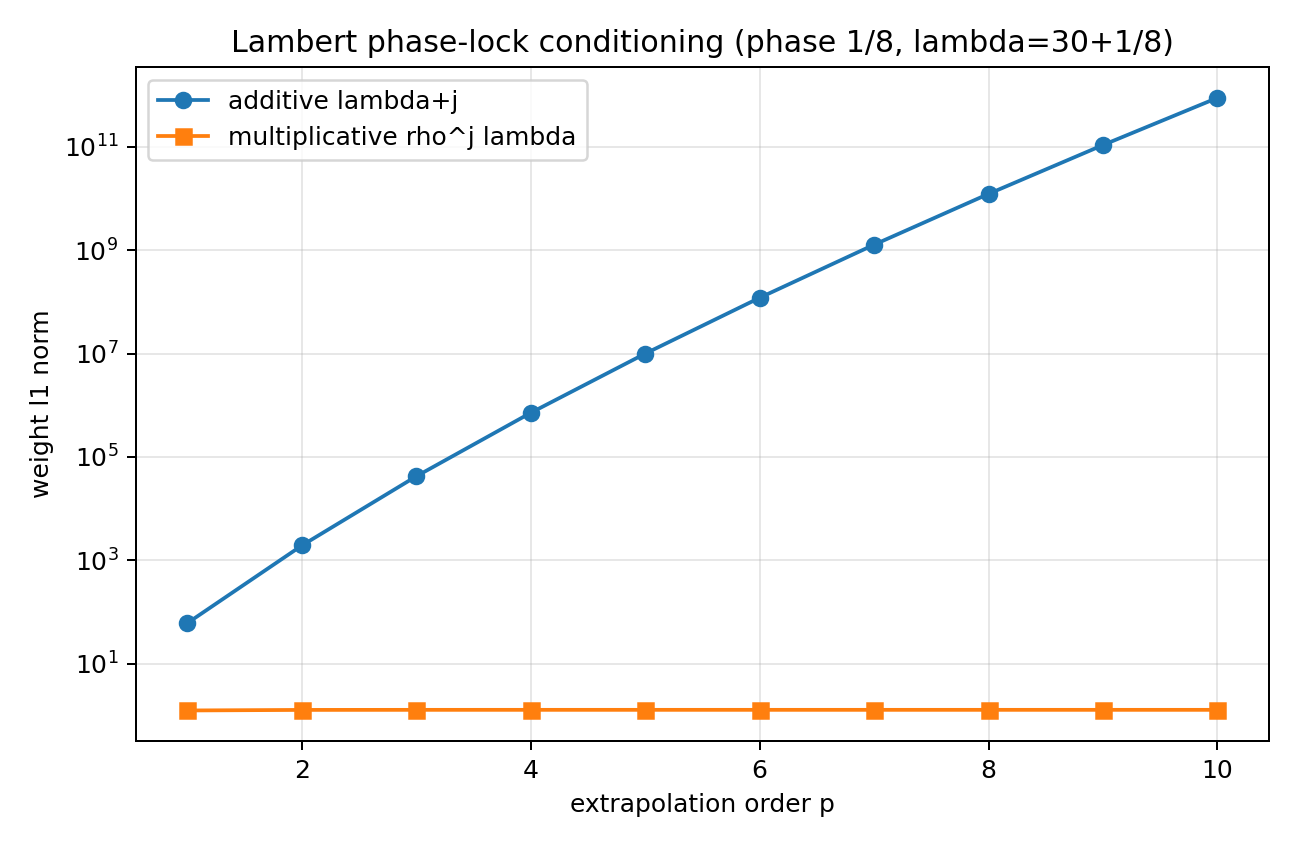
\includegraphics[width=0.80\textwidth]{lambert_conditioning.png}
\caption{Exact $\ell^1$ norms for additive and multiplicative phase-locked extrapolation.
The multiplicative row uses the rational phase $1/8$ and $\rho=9$.}
\label{fig:lambert-conditioning}
\end{figure}

\section{The maximal Gamma--zeta strip}
\label{sec:maximal-strip}

The exact mode formula \eqref{eq:gamma-zeta-coeff} contains more analytic information than
mere smoothness of the periodic term.

\subsection{Exact exponential type of the Fourier coefficients}

For $t>0$, the classical Gamma identity \cite{dlmf}
\begin{equation}
 |\Gamma(\ii t)|^2=\frac{\pi}{t\sinh(\pi t)}
 \label{eq:gamma-modulus}
\end{equation}
implies
\begin{equation}
 \log|\Gamma(\ii t)|
 =-\frac{\pi t}{2}-\frac12\log t+\frac12\log(2\pi)+o(1).
 \label{eq:gamma-log-asymptotic}
\end{equation}
Classical bounds on the line $\Re s=1$ \cite{titchmarsh,trudgian2014,trudgian2015} give
\begin{equation}
 |\zeta(1+\ii t)|\ll\log(2+t),
 \qquad
 |\zeta(1+\ii t)|^{-1}\ll\log(2+t),
 \label{eq:zeta-one-line-bounds}
\end{equation}
so $\log|\zeta(1+\ii t)|=o(t)$.

\begin{theorem}[exact Fourier exponential type]
\label{thm:coefficient-type}
Let $c_k$ be given by \eqref{eq:gamma-zeta-coeff}.  Then
\begin{equation}
 \boxed{\displaystyle
 \lim_{|k|\to\infty}-\frac{1}{|k|}\log|c_k|
 =\alpha:=\frac{\pi^2}{\log2}.}
 \label{eq:exact-coefficient-type}
\end{equation}
More quantitatively,
\begin{equation}
 |c_k|
 \ll\frac{\log(2+|k|)}{\sqrt{|k|}}
 \exp\!\left(-\frac{\pi^2}{\log2}|k|\right).
 \label{eq:coefficient-upper}
\end{equation}
\end{theorem}

\begin{proof}
For $k>0$, put $t_k=2\pi k/L$.  Equations
\eqref{eq:gamma-zeta-coeff}, \eqref{eq:gamma-log-asymptotic}, and
\eqref{eq:zeta-one-line-bounds} give
\[
 \log|c_k|=-\frac{\pi t_k}{2}+o(t_k)
 =-\frac{\pi^2}{L}k+o(k).
\]
The $k<0$ case follows by conjugation.  Keeping the elementary prefactor in
\eqref{eq:gamma-modulus} and the upper zeta bound gives
\eqref{eq:coefficient-upper}.
\end{proof}

\subsection{Maximal holomorphy}

\begin{theorem}[maximal horizontal strip]
\label{thm:maximal-strip}
The one-periodic function
\begin{equation}
 A_0(z)=c_0+\sum_{k\ne0}c_k\e^{2\pi\ii kz}
 \label{eq:periodic-fourier-series}
\end{equation}
extends holomorphically to
\begin{equation}
 \boxed{\displaystyle
 \mathcal S_*=
 \left\{z\in\C:\ |\Im z|<\sigma_*\right\},
 \qquad
 \sigma_*:=\frac{\pi}{2\log2}.}
 \label{eq:maximal-strip}
\end{equation}
It has no holomorphic continuation to any strictly wider horizontal strip.
\end{theorem}

\begin{proof}
If $|\Im z|<\sigma_*$, the extra Fourier factor has magnitude at most
$\exp(2\pi|k||\Im z|)$.  The upper bound \eqref{eq:coefficient-upper} makes the
series locally normally convergent because
$2\pi|\Im z|<\pi^2/L$.  Hence it is holomorphic in $\mathcal S_*$.

Suppose it continued to $|\Im z|<\sigma_*+\delta$.  Periodicity continues by the
identity theorem.  For $k>0$, shift the Fourier-coefficient contour to the compact line
$\Im z=-(\sigma_*+\delta/2)$.  Boundedness on one period gives
\[
 |c_k|\le C\exp\bigl(-2\pi(\sigma_*+\delta/2)k\bigr),
\]
contradicting \eqref{eq:exact-coefficient-type}, because $2\pi\sigma_*=\alpha$.
Shifting upward gives the same contradiction for negative modes.
\end{proof}

\begin{remark}
Maximality of the symmetric strip does not by itself prove that every point of either
boundary line is singular.  The stronger natural-boundary statement is a conjecture in
\cref{sec:open}.
\end{remark}

\begin{figure}[H]
\centering
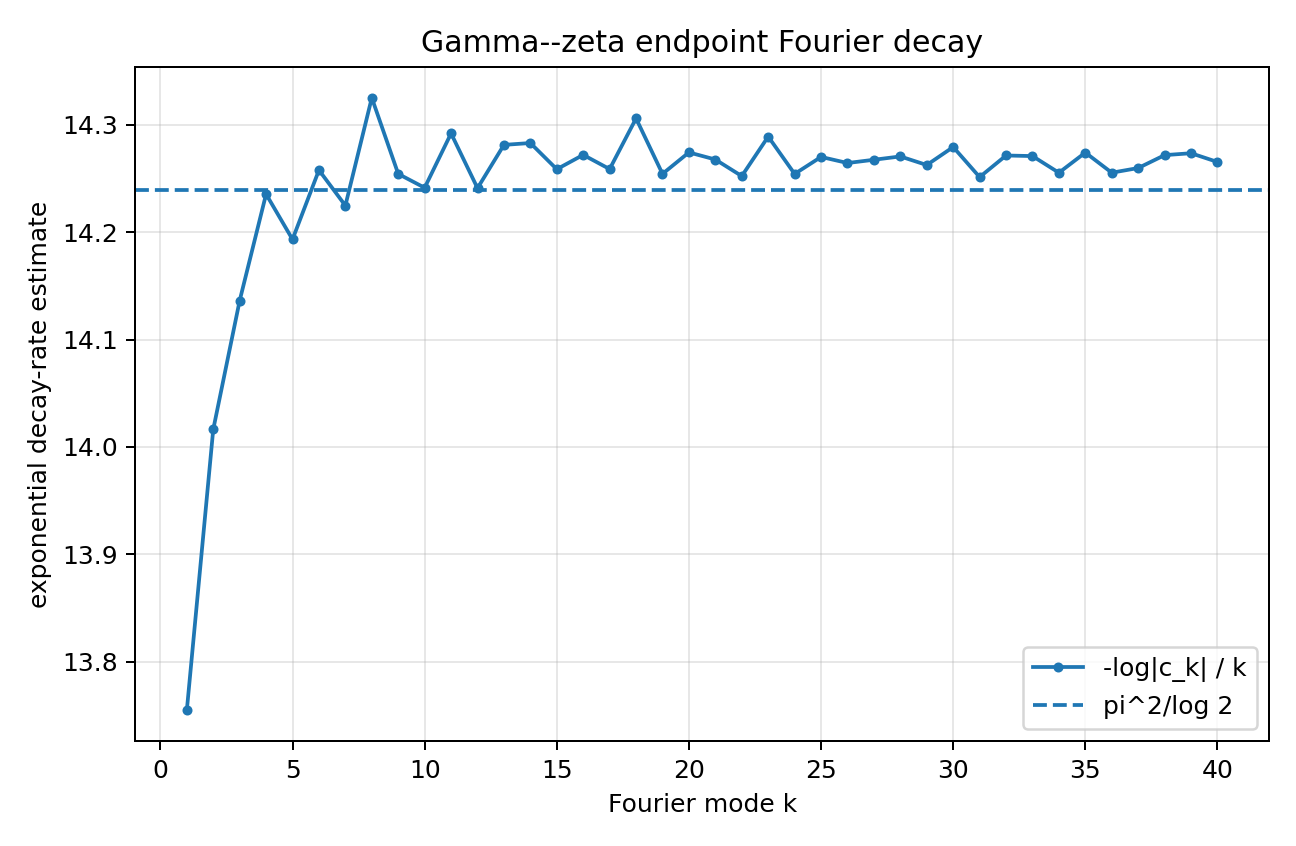
\includegraphics[width=0.80\textwidth]{gamma_zeta_decay.png}
\caption{High-precision values of $-\log|c_k|/k$ and the exact limiting constant
$\pi^2/\log2$.  Small oscillations come from the zeta factor; the Gamma factor fixes the
exponential rate.}
\label{fig:gamma-zeta-decay}
\end{figure}

\section{Weighted Wiener algebras and Bell-polynomial stability}
\label{sec:wiener}

The maximal strip gives quantitative control of every differential-polynomial periodic
coefficient built from $A_0$.

\begin{definition}
For $\sigma\ge0$, let $\Wiener_\sigma$ be the weighted Wiener algebra of one-periodic
Fourier series
\[
 f(z)=\sum_{k\in\Z}\widehat f(k)\e^{2\pi\ii kz},
 \qquad
 \|f\|_\sigma=\sum_{k\in\Z}|\widehat f(k)|\e^{2\pi\sigma|k|}<\infty.
\]
\end{definition}

\begin{theorem}[Wiener--Bell calculus]
\label{thm:wiener-bell}
Let $0\le\tau<\sigma$.
\begin{enumerate}
\item $\Wiener_\sigma$ is a Banach algebra and
$\|fg\|_\sigma\le\|f\|_\sigma\|g\|_\sigma$.
\item If $f\in\Wiener_\sigma$, then for $r\ge1$,
\begin{equation}
 \|f^{(r)}\|_\tau
 \le\left(\frac{r}{\e(\sigma-\tau)}\right)^r\|f\|_\sigma.
 \label{eq:derivative-wiener}
\end{equation}
\item If $S_Kf=\sum_{|k|\le K}\widehat f(k)\e^{2\pi\ii kz}$, then
\begin{equation}
 \sup_{|\Im z|\le\tau}|f(z)-S_Kf(z)|
 \le\e^{-2\pi(\sigma-\tau)(K+1)}\|f\|_\sigma.
 \label{eq:fourier-tail-wiener}
\end{equation}
\item For the complete exponential Bell polynomial $\Bell_n$ and
$f_1,\ldots,f_n\in\Wiener_\sigma$,
\begin{equation}
 \|\Bell_n(f_1,\ldots,f_n)\|_\sigma
 \le\Bell_n(\|f_1\|_\sigma,\ldots,\|f_n\|_\sigma).
 \label{eq:bell-wiener}
\end{equation}
In particular, if $g=\exp f$, then
\begin{equation}
 \|g^{(n)}\|_\tau
 \le \e^{\|f\|_\tau}
 \Bell_n\bigl(\|f'\|_\tau,\ldots,\|f^{(n)}\|_\tau\bigr).
 \label{eq:exp-bell-bound}
\end{equation}
\end{enumerate}
\end{theorem}

\begin{proof}
The product estimate is the weighted convolution inequality.  For derivatives, the
Fourier multiplier is $(2\pi\ii k)^r$, and
\[
 (2\pi x)^r\e^{-2\pi(\sigma-\tau)x}
 \le\left(\frac{r}{\e(\sigma-\tau)}\right)^r.
\]
The tail estimate follows by extracting the factor
$\e^{-2\pi(\sigma-\tau)(K+1)}$.  Complete Bell polynomials have nonnegative scalar
coefficients, so repeated use of the Banach-algebra inequality proves
\eqref{eq:bell-wiener}.  The last assertion is Fa\`a di Bruno's formula
$g^{(n)}=g\Bell_n(f',\ldots,f^{(n)})$ and
$\|\exp f\|_\tau\le\exp\|f\|_\tau$.
\end{proof}

\begin{corollary}[certified endpoint coefficient truncation]
\label{cor:certified-bell}
The leading Fabius endpoint fluctuation $A_0$ belongs to $\Wiener_\sigma$ for every
$\sigma<\sigma_*$.  Any coefficient obtained from finitely many derivatives, products,
Bell polynomials, and scalar Bernoulli constants belongs to the same family of algebras.
Its Fourier truncation error on every smaller strip is exponentially certified by
\eqref{eq:fourier-tail-wiener}.
\end{corollary}

This supplies a functional-analytic justification for a practical operation repeatedly
needed in the all-orders endpoint theory: compute a short Fourier representation of the
primitive periodic term, differentiate and combine it through Bell polynomials, and retain
rigorous control rather than relying only on pointwise numerical smallness.

\section{Radial--angular Lambert phase tomography}
\label{sec:tomography}

The multiplicative phase orbits recover values of periodic coefficient functions.  A phase
grid then recovers their Fourier spectra.

\subsection{Radial interpolation of the coefficient jet}

Fix a rational phase $\theta$, an admissible $\rho$, $q=\rho^{-1}$, and
$H=(n+\theta)^{-1}$.  Suppose
\begin{equation}
 y_s=\mathscr E(\rho^s(n+\theta))
 =\sum_{j=0}^{p}B_jq^{sj}+r_s,
 \qquad B_j=A_j(\theta)H^j.
 \label{eq:radial-polynomial-model}
\end{equation}
Let $\ell_s(t)$ be the Lagrange basis at the geometric nodes
$1,q,\ldots,q^p$:
\begin{equation}
 \ell_s(t)=\prod_{\substack{0\le r\le p\\r\ne s}}
 \frac{t-q^r}{q^s-q^r}.
 \label{eq:geometric-lagrange-basis}
\end{equation}
Define
\begin{equation}
 \widehat A_j(\theta)
 =H^{-j}[t^j]\sum_{s=0}^{p}y_s\ell_s(t).
 \label{eq:radial-jet-estimator}
\end{equation}

\begin{theorem}[radial jet recovery]
\label{thm:radial-jet}
If $r_s=0$, \eqref{eq:radial-jet-estimator} recovers
$A_0(\theta),\ldots,A_p(\theta)$ exactly.  In general,
\begin{equation}
 |\widehat A_j(\theta)-A_j(\theta)|
 \le H^{-j}\sum_{s=0}^{p}
 \left|[t^j]\ell_s(t)\right||r_s|.
 \label{eq:radial-jet-error}
\end{equation}
If $r_s=\bigO(H^{p+1}q^{s(p+1)})$ uniformly in phase, then
\begin{equation}
 \widehat A_j(\theta)-A_j(\theta)=\bigO(H^{p+1-j}).
 \label{eq:radial-jet-order}
\end{equation}
For $j=0$, the weights are exactly \eqref{eq:q-richardson-weights}.
\end{theorem}

\begin{proof}
The sample vector without remainders is the evaluation of the polynomial
$\sum_{j=0}^{p}B_jt^j$ at $t=q^s$.  Lagrange interpolation reconstructs it exactly.
Subtracting the remainder interpolant gives \eqref{eq:radial-jet-error}.  Since $p$ and
$q$ are fixed, the coefficient weights are fixed constants, proving
\eqref{eq:radial-jet-order}.
\end{proof}

The full coefficient weights also have a closed $q$-binomial form.  Put
$X_p=\{1,q,\ldots,q^p\}$.  The denominator is
\begin{equation}
 \prod_{r\ne s}(q^s-q^r)
 =(-1)^sq^{sp-s(s+1)/2}(q;q)_s(q;q)_{p-s},
 \label{eq:lagrange-denominator}
\end{equation}
and
\begin{equation}
 [t^j]\ell_s(t)
 =\frac{(-1)^{p-j}e_{p-j}(X_p\setminus\{q^s\})}
 {(-1)^sq^{sp-s(s+1)/2}(q;q)_s(q;q)_{p-s}}.
 \label{eq:jet-q-weights}
\end{equation}
The excluded elementary symmetric polynomial can be reduced to Gaussian binomials through
\begin{equation}
 e_m(X_p\setminus\{q^s\})
 =\sum_{a=0}^{m}(-q^s)^a
 q^{(m-a)(m-a-1)/2}\qbinom{p+1}{m-a}{q}.
 \label{eq:excluded-e-qbinom}
\end{equation}
Thus the entire radial coefficient jet is governed by the same $q$-binomial algebra as the
zeroth-order Richardson row.

\subsection{Angular DFT and exact aliasing}

Let a one-periodic coefficient have an absolutely convergent Fourier expansion
\begin{equation}
 A(u)=\sum_{k\in\Z}c_k\e^{2\pi\ii ku}.
 \label{eq:A-fourier}
\end{equation}
Sample it at the rational phases $u_r=r/d$ and define
\begin{equation}
 \widetilde c_k^{(d)}
 =\frac1d\sum_{r=0}^{d-1}A(r/d)\e^{-2\pi\ii kr/d}.
 \label{eq:dft-estimator}
\end{equation}

\begin{theorem}[exact phase alias identity]
\label{thm:phase-alias}
For every integer $k$,
\begin{equation}
 \boxed{\displaystyle
 \widetilde c_k^{(d)}=\sum_{m\in\Z}c_{k+md}.}
 \label{eq:phase-alias}
\end{equation}
If, for some $\beta>0$, $|c_k|\le C\e^{-\beta|k|}$ and
$|k|\le(d-1)/2$, then
\begin{equation}
 |\widetilde c_k^{(d)}-c_k|
 \le\frac{2C\e^{-\beta(d-|k|)}}{1-\e^{-\beta d}}.
 \label{eq:alias-bound}
\end{equation}
\end{theorem}

\begin{proof}
Insert \eqref{eq:A-fourier} into \eqref{eq:dft-estimator}.  The finite geometric
sum is one precisely when the Fourier index is congruent to $k$ modulo $d$, and zero
otherwise.  For the bound, every nonprincipal alias satisfies
$|k+md|\ge |m|d-|k|$; sum the two geometric tails.
\end{proof}

By \cref{thm:coefficient-type}, for every $\varepsilon>0$ the Fabius coefficients obey
$|c_k|\le C_\varepsilon\exp[-(\alpha-\varepsilon)|k|]$.  Hence the DFT alias error has the
sharp available exponential scale $\alpha=\pi^2/L$.

\subsection{The combined tomography theorem}

\begin{theorem}[two-axis Lambert phase tomography]
\label{thm:two-axis}
Let $d\ge2$, choose $\rho\equiv1\pmod d$, and use the radial order-$p$ estimator at each
phase $r/d$.  Suppose the normalized endpoint residual has the uniform expansion
\eqref{eq:pure-endpoint-expansion} through order $p+1$, and suppose
$A_0\in\Wiener_\sigma$ for some $\sigma>0$.  For
$|k|\le(d-1)/2$, the DFT of the radial estimates satisfies
\begin{equation}
 \widehat c_{k}^{(d,p,n)}-c_k
 =\bigO(n^{-p-1})
 +\bigO\!\left(\e^{-2\pi\sigma(d-|k|)}\right),
 \label{eq:two-axis-error}
\end{equation}
uniformly over the phase grid.  For the leading Fabius periodic term one may take every
$\sigma<\pi/(2L)$, so the angular exponent can be made arbitrarily close to
$\pi^2/L$.
\end{theorem}

\begin{proof}
Equation \eqref{eq:multiplicative-leading-error} gives a uniform
$\bigO(n^{-p-1})$ error at each phase.  Averaging by a DFT does not increase the maximum
absolute error.  Apply \cref{thm:phase-alias} to the exact phase values, with the Fourier
bound supplied by membership in $\Wiener_\sigma$.
\end{proof}

The same construction applies to every $A_j$: use the full radial jet estimator
\eqref{eq:radial-jet-estimator}, then a DFT in the phase variable.  By
\cref{cor:certified-bell}, periodic coefficients formed through the audited
Bell/Bernoulli saddle calculus inherit exponentially controlled phase spectra.

\begin{figure}[H]
\centering
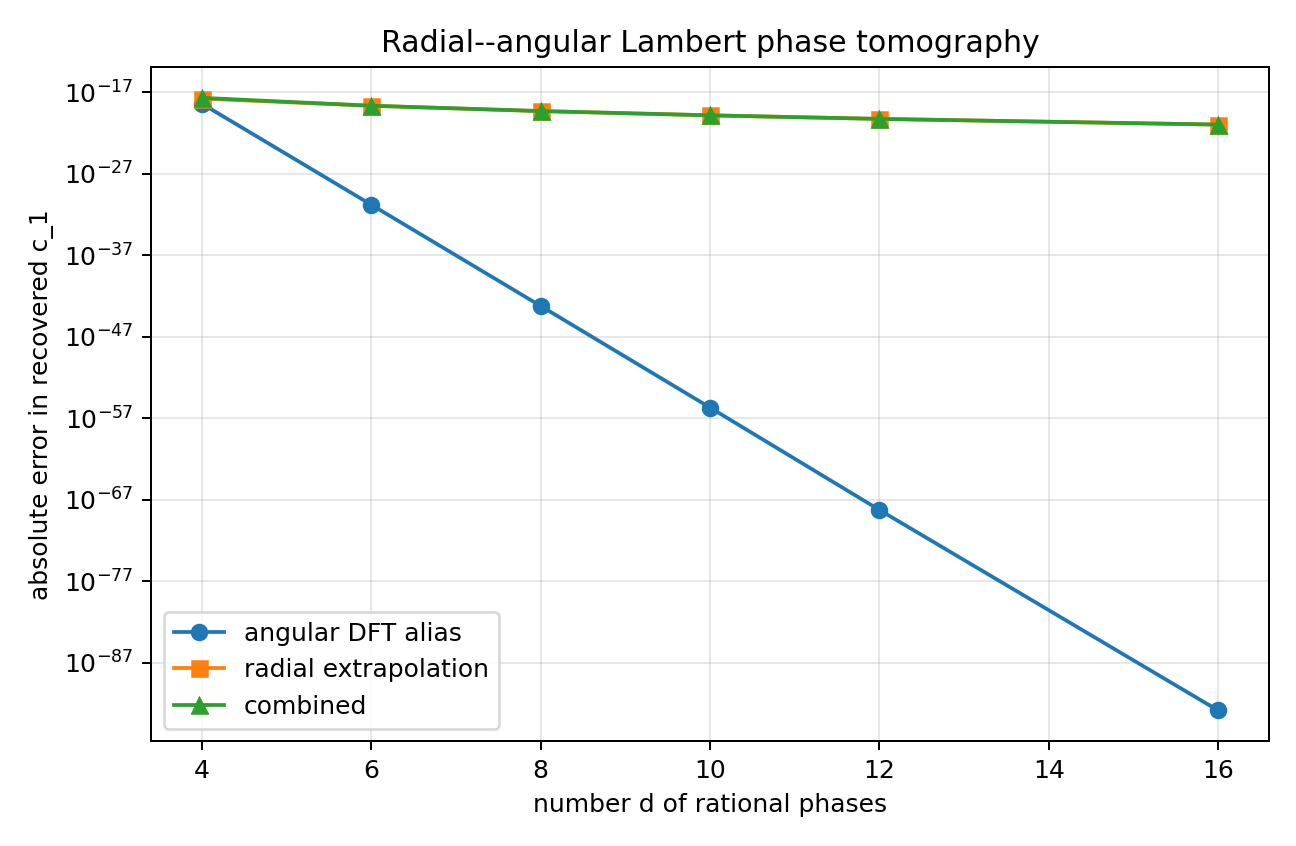
\includegraphics[width=0.80\textwidth]{tomography_errors.png}
\caption{A controlled two-axis experiment recovering $c_1$.  The angular samples use the
actual Gamma--zeta periodic term; documented smooth surrogate functions supply higher
inverse-Lambert coefficients so that the radial cancellation can be tested independently.}
\label{fig:tomography}
\end{figure}

\section{Numerical and exact-arithmetic experiments}
\label{sec:experiments}

The accompanying \path{numerical_experiments.py} is deliberately independent of the
LaTeX source.  It uses exact \texttt{Fraction} arithmetic for all polynomial filters and
90-decimal-digit \texttt{mpmath} arithmetic for Gamma--zeta calculations.  The zeta
function is forced to use Euler--Maclaurin evaluation rather than an automatic method
selection, avoiding threshold-dependent loss of reproducibility on the line $\Re s=1$.

\subsection{Exact filter verification}

For $q=1/2$ and every order $1\le m\le10$, the script checks
\[
 \sum_jw_j(N+j)^\ell q^{N+j}=0,
 \qquad 0\le\ell<m,
\]
for both the minimal and twisted Thue--Morse filters.  Every residual is an exact rational
zero.  It also verifies the mixed filter \eqref{eq:mixed-filter}.

\begin{table}[H]
\centering
\caption{Span--conditioning tradeoff at $q=1/2$.}
\label{tab:filter-conditioning}
\begin{tabular}{rrrrr}
\toprule
$m$ & minimal span & minimal $\kappa$ & TM span & TM $\kappa$\\
\midrule
1 & 1 & 3 & 1 & 3.0000000000\\
2 & 2 & 9 & 3 & 5.0000000000\\
3 & 3 & 27 & 7 & 5.6666666667\\
4 & 4 & 81 & 15 & 5.7111111111\\
5 & 5 & 243 & 31 & 5.7112854031\\
6 & 6 & 729 & 63 & 5.7112854057\\
8 & 8 & 6561 & 255 & 5.7112854057\\
10 & 10 & 59049 & 1023 & 5.7112854057\\
\bottomrule
\end{tabular}
\end{table}

\begin{figure}[H]
\centering
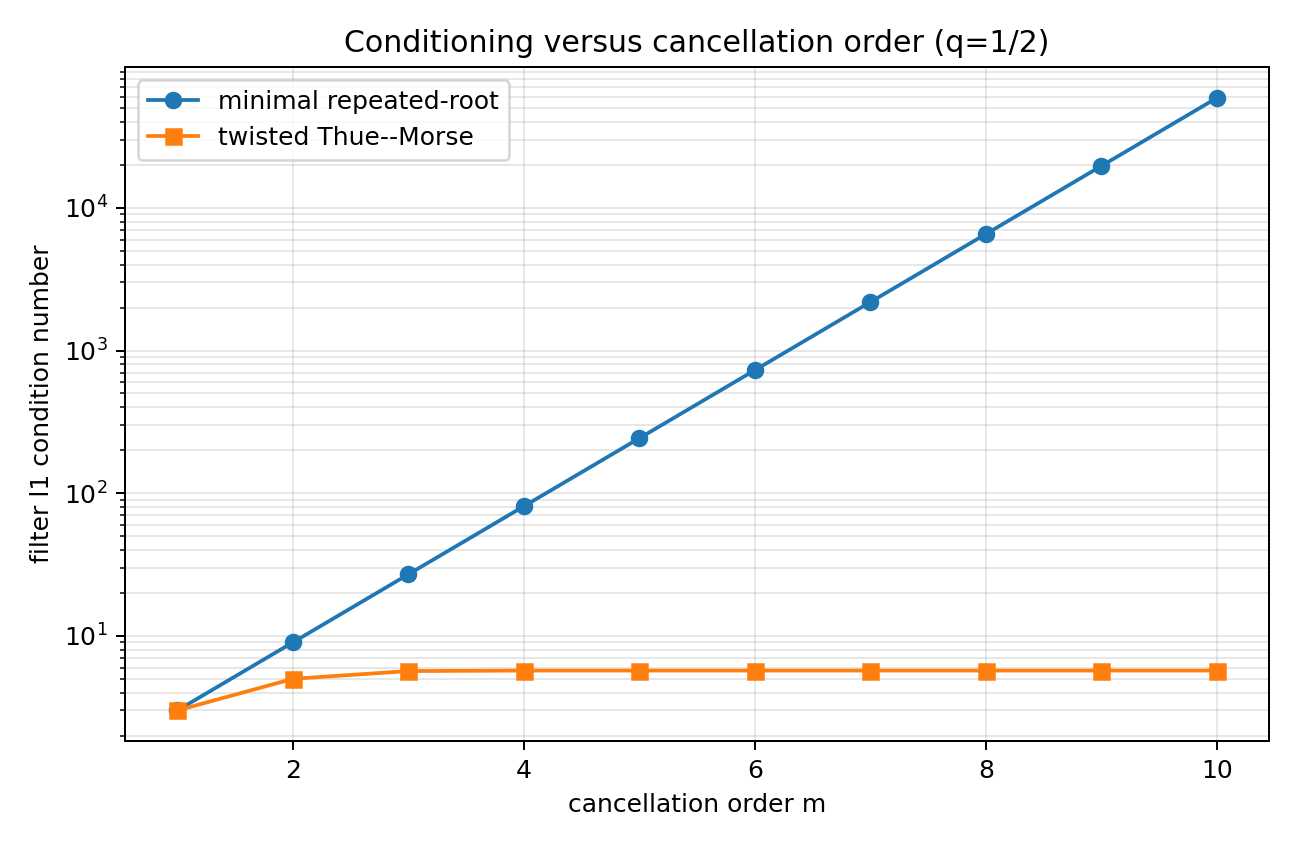
\includegraphics[width=0.80\textwidth]{conditioning_tradeoff.png}
\caption{Minimal repeated-root and twisted Thue--Morse condition numbers.  The vertical
axis is logarithmic; the digital curve rapidly approaches its finite limit.}
\label{fig:conditioning-tradeoff}
\end{figure}

\subsection{Gamma--zeta modes}

The first nonzero modes are:
\begin{table}[H]
\centering
\caption{High-precision magnitudes of the endpoint Fourier coefficients.}
\label{tab:gamma-zeta}
\begin{tabular}{rcc}
\toprule
$k$ & $|c_k|$ & $-\log|c_k|/k$\\
\midrule
1 & $1.06271162518632\times10^{-6}$ & 13.7546867793\\
2 & $6.69278636792434\times10^{-13}$ & 14.0162879620\\
3 & $3.82107872358669\times10^{-19}$ & 14.1361946653\\
4 & $1.86460518002229\times10^{-25}$ & 14.2353944985\\
5 & $1.51268570169932\times10^{-31}$ & 14.1932502403\\
10 & $1.41459209881527\times10^{-62}$ & 14.2413434545\\
\bottomrule
\end{tabular}
\end{table}
The exact limiting rate is
\[
 \alpha=14.2388293249875054338606757113\ldots,
 \qquad
 \sigma_*=2.26618007091359690481384147286\ldots.
\]

\subsection{Tomography experiment}

The angular part evaluates the actual truncated Gamma--zeta series for $A_0$.  To test
radial cancellation without silently importing unparsed formulas for the higher audited
saddle coefficients, the program defines explicit smooth surrogate coefficients
\[
 \widehat A_j(k)=0.2^j\left(1+\frac{k^2}{(j+1)^2}\right)c_k,
 \qquad j\ge1.
\]
This surrogate has the same real symmetry and strip structure; it is not claimed to equal
the true $A_j$.  Radial order $p=3$, starting integer $n=16$, and $\rho=d+1$ give:

\begin{table}[H]
\centering
\caption{Recovery error for $c_1$ in the controlled radial--angular model.}
\label{tab:tomography}
\begin{tabular}{rrrr}
\toprule
$d$ & angular alias & radial error & combined error\\
\midrule
4 & $3.8211\times10^{-19}$ & $1.6041\times10^{-18}$ & $1.9862\times10^{-18}$\\
6 & $1.5127\times10^{-31}$ & $2.1303\times10^{-19}$ & $2.1303\times10^{-19}$\\
8 & $5.7018\times10^{-44}$ & $4.7054\times10^{-20}$ & $4.7054\times10^{-20}$\\
10 & $1.9284\times10^{-56}$ & $1.4089\times10^{-20}$ & $1.4089\times10^{-20}$\\
12 & $5.2972\times10^{-69}$ & $5.1635\times10^{-21}$ & $5.1635\times10^{-21}$\\
16 & $1.2993\times10^{-93}$ & $1.0305\times10^{-21}$ & $1.0305\times10^{-21}$\\
\bottomrule
\end{tabular}
\end{table}

The exact rational phase drift is zero in every sample.  Once $d\ge6$, angular aliasing is
negligible relative to the order-three radial remainder, exactly as
\eqref{eq:two-axis-error} predicts.

\section{Consequences for the Fabius--Rvachev research program}
\label{sec:consequences}

\subsection{A single annihilator language}

Three constructions that look unrelated become instances of one spectral polynomial.
\begin{enumerate}
\item Ordinary Richardson extrapolation puts simple roots at the known error ratios.
\item Confluent Richardson puts repeated roots at ratios carrying polynomial prefactors.
\item Prouhet--Thue--Morse cancellation is a digitally factorized repeated root, with the
      exponential twist chosen so that the geometric factor cancels before the Prouhet sum
      is taken.
\end{enumerate}
This shift-polynomial language is especially convenient for Lean: the analytic application
is reduced to a finite polynomial divisibility lemma plus a norm estimate.

\subsection{Endpoint coefficient spectroscopy}

The exact-Lambert phase is not only an asymptotic bookkeeping device.  Rational
multiplicative orbits turn the endpoint into a laboratory in which one may recover the
periodic coefficient functions $A_j$ separately.  A practical high-precision workflow is:
\begin{enumerate}
\item choose a phase denominator $d$ and $\rho\equiv1\pmod d$;
\item evaluate the normalized log Fabius residual at
$x_{r,s}=\lambda_{r,s}2^{-\lambda_{r,s}}$, where
$\lambda_{r,s}=\rho^s(n+r/d)$;
\item perform radial $q$-interpolation to recover $A_j(r/d)$;
\item perform a DFT over $r$ to recover Fourier coefficients;
\item certify radial error from the next asymptotic order and angular error from the
      Wiener strip.
\end{enumerate}
The method applies equally to coefficients in the inverse-Fabius endpoint expansion once
the corresponding normalized residual is written in the exact Lambert coordinate.

\subsection{Bell and Bernoulli closure}

The corpus's Bell-polynomial coefficient calculus often makes formulas look combinatorially
explosive.  In the weighted Wiener algebra, however, every product and Bell composition is
norm-submultiplicative.  Bernoulli numbers enter as scalar coefficients, while derivatives
are controlled by the strip margin.  This suggests a certified implementation architecture:
store periodic functions as weighted Fourier vectors, build each all-orders coefficient by
Bell operations, and propagate a scalar norm bound in parallel.  Numerical truncation then
comes with a theorem-level remainder certificate.

\subsection{Generalized Pascal--Rvachev hierarchies}

Higher-rank Mellin poles naturally produce polynomial factors in the logarithmic scale.
Along a multiplicative phase orbit these are exactly the $s^\ell q^{rs}$ modes treated by
confluence.  The digital filter is therefore likely to be more useful for the hierarchy
than for the classical rank-one case: higher pole orders increase confluence, and the
minimal filter's condition number grows exponentially in that order, while a digital
factorization can keep it bounded.

\section{Conjectures and promising research directions}
\label{sec:open}

\begin{conjecturebox}{Conjecture 1: natural boundary of the endpoint fluctuation}
The two lines
\[
 \Im z=\pm\frac{\pi}{2\log2}
\]
are natural boundaries for the leading periodic endpoint function $A_0$.  The maximal-strip
theorem proves that some obstruction occurs at each side, but does not locate the singular
set.  A route to proof is to analyze the phase of
$\Gamma(-\chi_k)\zeta(1-\chi_k)$ and apply a gap-free natural-boundary criterion for Fourier
series of exact exponential type.
\end{conjecturebox}

\begin{conjecturebox}{Conjecture 2: sharp DFT alias exponent}
For every fixed nonzero mode $k$, the exact phase-grid alias
$\sum_{m\ne0}c_{k+md}$ satisfies
\[
 \log\left|\sum_{m\ne0}c_{k+md}\right|
 =-\frac{\pi^2}{\log2}d+o(d)
\]
outside, at most, a sparse exceptional set of grid sizes.  The upper exponential rate is
proved here; the issue is ruling out systematic phase cancellation among the nearest aliases.
\end{conjecturebox}

\begin{problem}[optimal span--conditioning frontier]
For $q\in(0,1)$ define
\[
 K_m(q;D)=\inf\left\{\sum_{j=0}^{D}|w_j|:
 W(1)=1,\ (z-q)^m\mid W(z),\ \deg W\le D\right\}.
\]
Determine $K_m(q;D)$ uniformly between the endpoints
\[
 K_m(q;m)=\left(\frac{1+q}{1-q}\right)^m,
 \qquad
 \inf_DK_m(q;D)=1.
\]
The Prouhet factorizations provide explicit upper bounds.  The binary choice is uniquely
minimal-span among collision-free complete digital stencils, but the full Pareto frontier
appears to be a nontrivial extremal problem in polynomial approximation and linear
programming.
\end{problem}

\begin{problem}[irrational near-locks]
For irrational phase $\theta$, exact multiplicative locks do not exist.  Continued-fraction
approximants can choose $\rho$ with $\|(\rho-1)\theta\|$ small, but the phase defect is
multiplied by $1+\rho+\cdots+\rho^{s-1}$.  Develop a simultaneous Diophantine criterion that
balances this phase drift against the bounded Richardson weights and the strip-controlled
phase derivative.  The expected result is a provable work--accuracy tradeoff for irrational
phase tomography.
\end{problem}

\begin{conjecturebox}{Conjecture 3: common strip in the Pascal--Rvachev hierarchy}
After subtraction of the rank-dependent logarithmic polynomial, every periodic coefficient
in the Pascal--Rvachev endpoint hierarchy has maximal strip half-width
$\pi/(2\log2)$.  Higher rank changes only polynomial factors in the Fourier mode and hence
the boundary singularity order, not the Gamma-controlled exponential type.
\end{conjecturebox}

\begin{conjecturebox}{Conjecture 4: boundary singularities control late Bell coefficients}
The large-order growth of the all-orders endpoint and inverse-endpoint Bell-polynomial
coefficients is governed by the nearest singularities on the two strip boundaries.  After
appropriate normalization, the coefficient sequence should admit a resurgent
factorial-over-power law with phase determined by the boundary singularities.  Establishing
this would connect the exact Gamma--zeta Fourier spectrum to optimal truncation and
exponentially improved Lambert asymptotics.
\end{conjecturebox}

\subsection{A concrete Lean formalization order}

The new results break naturally into short formal modules.
\begin{enumerate}
\item Define polynomial shift operators on sequences valued in a normed additive group.
\item Prove \cref{lem:shift-euler} for scalar geometric-polynomial modes.
\item Formalize root multiplicity, the minimal annihilator, and the finite norm bound.
\item Import the existing finite Thue--Morse polynomial and prove
$\mathcal T_{m,q}=T_m(z/q)/T_m(1/q)$, coefficient formula
\eqref{eq:tm-filter-coeff}, and norm formula \eqref{eq:tm-condition}.
\item Prove the modular arithmetic phase lock \cref{thm:multiplicative-lock} over rationals.
\item Reuse the existing Gaussian $q$-binomial Lagrange development for the radial jet.
\item Formalize the finite DFT alias identity; postpone the complex-analytic maximal-strip
      theorem until Gamma and zeta estimates are available in the chosen library layer.
\end{enumerate}
The first six items are predominantly finite algebra and should be substantially easier than
the endpoint analytic inputs already present in the project.

\section{Conclusion}

The main structural discovery is not another isolated formula for $F$, $F^{-1}$, or
$\widehat\Up$.  It is a reusable spectral calculus.

A root of a shift polynomial represents an asymptotic geometric mode; multiplicity
represents its polynomial decoration.  The standard $q$-Richardson row uses simple roots.
Confluence handles logarithmic and polynomial decorations.  A Thue--Morse product spreads a
repeated root over a binary stencil, exchanging span for bounded conditioning.  The exact
Lambert coordinate turns rational endpoint phases into geometric orbits on which those
filters act.  Finally, the Gamma--zeta mode formula supplies the sharp analytic strip needed
to reconstruct the phase dependence by DFT and to certify every subsequent Bell-polynomial
operation.

This package gives both theorem-level results and a practical experimental protocol.  It
also identifies clear next targets: the span--conditioning extremal problem, natural
boundaries, irrational phase locks, hierarchy-wide strip theorems, and resurgent late-order
analysis.  Each direction is tightly connected to existing formalized or audited machinery,
while avoiding duplication of the substantial frontier results already present in the
repository.

\appendix

\section{Auxiliary identities}
\label{app:identities}

\subsection{Complete homogeneous form of transformed moments}

For the geometric Lagrange weights, let
\[
 \mu_{p,r}(q)=\sum_{s=0}^{p}\omega_{p,s}(q)q^{sr}.
\]
Then $\mu_{p,0}=1$, $\mu_{p,r}=0$ for $1\le r\le p$, and for $r\ge p+1$,
\begin{equation}
 \mu_{p,r}(q)
 =(-1)^pq^{p(p+1)/2}
 h_{r-p-1}(1,q,\ldots,q^p),
 \label{eq:complete-homogeneous-moment}
\end{equation}
where $h_j$ is the complete homogeneous symmetric polynomial.  The identity follows from
the remainder of interpolation of $t^r$ at $1,q,\ldots,q^p$.  The standard specialization
\[
 h_{r-p-1}(1,q,\ldots,q^p)=\qbinom{r-1}{p}{q}
\]
recovers \eqref{eq:q-moment-transform}.

\subsection{Additive phase weights}

For completeness, the derivation of \eqref{eq:additive-weights} is one line.  At nodes
$h_j=(\lambda+j)^{-1}$, the Lagrange weight at zero is
\[
 \prod_{r\ne j}\frac{-h_r}{h_j-h_r}
 =\prod_{r\ne j}\frac{-(\lambda+j)}{r-j}
 =\frac{(-1)^{p-j}(\lambda+j)^p}{j!(p-j)!}.
\]
This exact formula makes the conditioning contrast transparent; it is not a numerical
artifact of solving a Vandermonde system.

\subsection{Digital condition limit}

The finite identity
\[
 \prod_{j=0}^{m-1}(1+q^{2^j})=\frac{1-q^{2^m}}{1-q}
\]
is simply the binary factorization of $1-q^{2^m}$.  Dividing by
$\Theta_m(q)$ gives \eqref{eq:tm-condition}; monotone convergence of
$\Theta_m(q)$ gives \eqref{eq:tm-condition-limit}.

\section{Reproduction guide}
\label{app:reproduction}

From the extracted report directory, run
\begin{lstlisting}[style=code]
python numerical_experiments.py --output-dir . --precision 90
latexmk -pdf -interaction=nonstopmode -halt-on-error fabius_frontier_report.tex
\end{lstlisting}
The script regenerates:
\begin{itemize}
\item \path{filter_conditioning.csv} and \path{conditioning_tradeoff.png};
\item \path{lambert_conditioning.csv} and \path{lambert_conditioning.png};
\item \path{gamma_zeta_coefficients.csv} and \path{gamma_zeta_decay.png};
\item \path{tomography_errors.csv} and \path{tomography_errors.png};
\item \path{experiment_results.txt} and \path{verification.json}.
\end{itemize}
Exact filter checks use Python's \texttt{Fraction}; no tolerance is involved.  Floating
experiments use \texttt{mpmath}.  The source comments document the surrogate higher endpoint
coefficients and every normalization.

\section{Complete pinned LaTeX inventory}
\label{app:inventory}

The following manifest is included as a separate plain-text file in the archive.  It records
the complete recursive 78-path corpus boundary used for the nonduplication audit.

\lstinputlisting[
  basicstyle=\ttfamily\scriptsize,
  breaklines=true,
  breakatwhitespace=false,
  frame=single,
  columns=fullflexible,
  keepspaces=true,
  showstringspaces=false
]{corpus_manifest.txt}

\begin{thebibliography}{99}

\bibitem{arias1982}
J. Arias de Reyna,
\newblock An infinitely differentiable function with compact support: definition and properties,
\newblock unpublished/translated source represented in the audited repository; original work from 1982.

\bibitem{arias2017}
J. Arias de Reyna,
\newblock Arithmetic of the Fabius function,
\newblock \emph{Annales de l'Institut Fourier} \textbf{67} (2017), 637--678.

\bibitem{aistleitner2015}
C. Aistleitner, R. Hofer, and G. Larcher,
\newblock On parametric Thue--Morse sequences and lacunary trigonometric products,
\newblock arXiv:1502.06738 (2015); source TeX represented in the audited repository.

\bibitem{alloucheshallit}
J.-P. Allouche and J. Shallit,
\newblock \emph{Automatic Sequences: Theory, Applications, Generalizations},
\newblock Cambridge University Press, 2003.

\bibitem{corless1996}
R. M. Corless, G. H. Gonnet, D. E. G. Hare, D. J. Jeffrey, and D. E. Knuth,
\newblock On the Lambert $W$ function,
\newblock \emph{Advances in Computational Mathematics} \textbf{5} (1996), 329--359.

\bibitem{sidi2006}
A. Sidi,
\newblock The Richardson extrapolation process with a harmonic sequence of collocation points,
\newblock \emph{SIAM Journal on Numerical Analysis} \textbf{37} (2000), 1729--1746.

\bibitem{titchmarsh}
E. C. Titchmarsh, revised by D. R. Heath-Brown,
\newblock \emph{The Theory of the Riemann Zeta-Function}, second edition,
\newblock Oxford University Press, 1986.

\bibitem{trudgian2014}
T. Trudgian,
\newblock A new upper bound for $|\zeta(1+it)|$,
\newblock \emph{Bulletin of the Australian Mathematical Society} \textbf{89} (2014), 259--264.

\bibitem{trudgian2015}
T. Trudgian,
\newblock Explicit bounds on the logarithmic derivative and the reciprocal of the Riemann zeta-function,
\newblock \emph{Functiones et Approximatio Commentarii Mathematici} \textbf{52} (2015), 253--261.

\bibitem{dlmf}
NIST Digital Library of Mathematical Functions,
\newblock Chapters 5 and 25: Gamma and Riemann zeta functions,
\newblock \url{https://dlmf.nist.gov/}.

\bibitem{proveit}
V. Reshetnikov,
\newblock \repo{}: Fabius-function formalization and documentation corpus,
\newblock pinned commit \texttt{f49aad5c9c6d627a64822ea9f8e46f5270b95cef}, 27 August 2026.

\end{thebibliography}

\end{document}
